\chapter{Implementación}

\section{Introducción}
\label{sec:intro}

Para la extracción de datos se ha utilizado, como se ha mencionado anteriormente, el plugin de recuperación de datos de Twitter para Gephi, introduciendo como cadenas de búsqueda las siguientes cadenas:

\begin{itemize}
	\item antonio mercero
	\item farmacia de guardia
	\item verano azul
	\item chanquete
\end{itemize}

\section{Estructura de la red}

En la red extraída los nodos son los usuarios (con información adicional como su número de seguidores, de usuarios que siguen, tuits o tuits marcados como favoritos) y las aristas son la interacción entre usuarios (mención, respuesta o retuit), por tanto se trata de una red dirigida.
\\ \\
La red original consta de 3693 nodos y 5845 aristas. Aplicando un primer filtro de componente gigante para deshacerse de grupos pequeños que no interaccionan con el grupo más grande, pasamos a 2627 nodos y 4720 aristas (el 71,13\% y 80,75\% respectivamente con respecto a la red social original).
\\ \\
A continuación se ha aplicado un filtro de \textit{k-core} con grado 3 para seguir simplificándola pues seguía siendo todavía demasiado grande y difícil de visualizar. Aplicando este filtro pasamos a 599 nodos y 1697 aristas (el 16,22\% y 29,03\% respectivamente con respecto a la red social original).

\section{Valores de medidas de análisis}
\label{sec:medidas}

\subsection{Red original}

\begin{figure}[H]
	\centering
	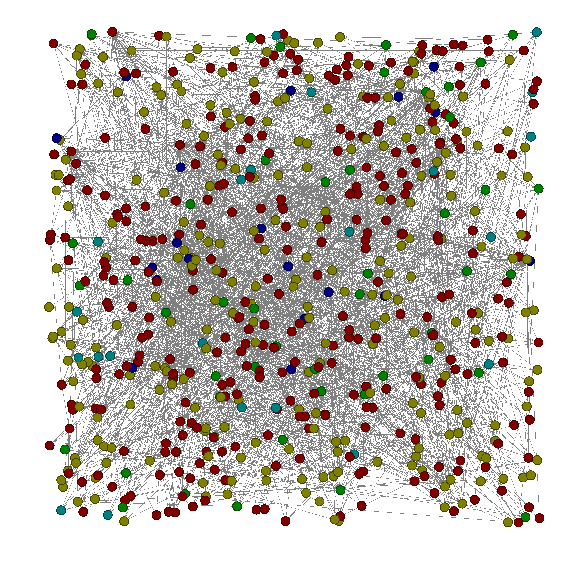
\includegraphics[width=12cm]{../images/original-graph}
	\caption{Grafo de la red original}
\end{figure}

\begin{table}[H]
	\centering
	\caption{Valores de las medidas de análisis de la red original}
	\label{tab:medidas-original}
	\begin{tabular}{| l | l |}
		\hline
		Medida                							& Valor          \\ 
		\hline
		Número de nodos ($N$)           					& 3693           \\
		Número de enlaces ($L$)                   		& 5845           \\
		Densidad ($D$)                   				& 0         \\
		Grado medio ($k$)                   				& 1,583          \\
		Diámetro ($d_{max}$)             				& 4              \\
		Distancia media ($d$)                   			& 1,642          \\
		Coeficiente clustering medio($C$)              	& 0,074          \\
		Componentes conexas   							& 9            \\ 
		Nodos componente gigante($N_{gigante}$)        	& 2627 (71,13\%) \\ 
		Enlaces componente gigante($L_{gigante}$)       & 4720 (80,75\%) \\ 
		\hline
	\end{tabular}
\end{table}

La densidad de la red original es muy pequeña (0). Vemos que hay casi el mismo número de nodos que de enlaces, ya que muchos usuarios solo mencionan el suceso sin realizar ninguna interacción con nadie.
\\ \\
La distancia media de un nodo a otro es muy pequeña lo cual es lógico al haber nodos que están conectados con un enorme número de usuarios. Además, el diámetro es de tan solo 4, por lo que, como muchos en 4 pasos, se podría pasar de un nodo a cualquier otro.
\\ \\
El coeficiente de clustering medio es muy bajo. Y es que como podemos ver hay hasta 9 componentes conexas lo cual puede explicar este valor tan bajo. En muchos casos es debido a usuarios que responden a otros usando el \textit{hash tag} sin mencionar a ningún otro usuario.

\subsection{Red filtrada}

\begin{figure}[H]
	\centering
	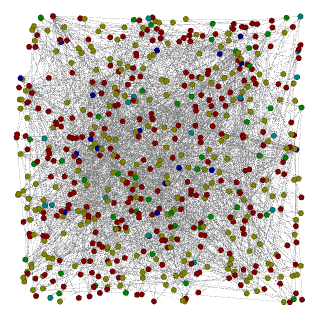
\includegraphics[width=12cm]{../images/filtered-graph}
	\caption{Grafo de la red filtrada}
\end{figure}

\begin{table}[H]
	\centering
	\caption{Valores de las medidas de análisis de la red filtrada}
	\label{tab:medidas-filtrada}
	\begin{tabular}{| l | l |}
		\hline
		Medida                							& Valor          \\ 
		\hline
		Número de nodos ($N$)           					& 599           \\
		Número de enlaces ($L$)                   		& 1697           \\
		Densidad ($D$)                   				& 0,005         \\
		Grado medio ($k$)                   				& 2,833          \\
		Diámetro ($d_{max}$)             				& 3              \\
		Distancia media ($d$)                   			& 1,431          \\
		Coeficiente clustering medio($C$)               & 0,003             \\
		Componentes conexas   					   		& 1            \\ 
		\hline
	\end{tabular}
\end{table}

La densidad sigue siendo pequeña pero es bastante mayor que la de la red original ya que ha pasado de 0 a 0,005.
\\ \\
La distancia varía de la red original a la filtrada, aumentando en 0,211, mientras que el diámetro se ha reducido a 3.
\\ \\
El coeficiente de \textit{clustering} sigue siendo bastante pequeño, lo cual puede hacer difícil la detección de comunidades para un número de comunidades pequeña.
\\ \\
En este caso, al haberse filtrado la red previamente usando la componente gigante, el número de componentes conexas es 1, como no podría ser de otra manera.

\section{Propiedades de la red}

A continuación se describirán propiedades de la red ya filtrada, que será sobre la que se haga la detección de comunidades y visualización.

\subsection{Distribución de grados}

\begin{figure}[H]
	\centering
	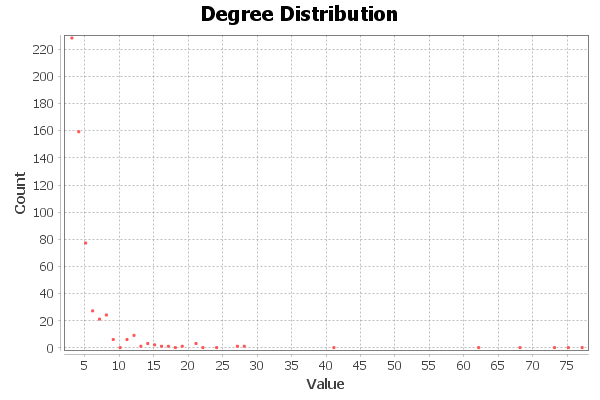
\includegraphics[width=12cm] {../images/degree-distribution}
	\caption{Distribución de grados para la red filtrada}
	\label{fig:degree-distribution}
\end{figure}

\begin{figure}[H]
	\centering
	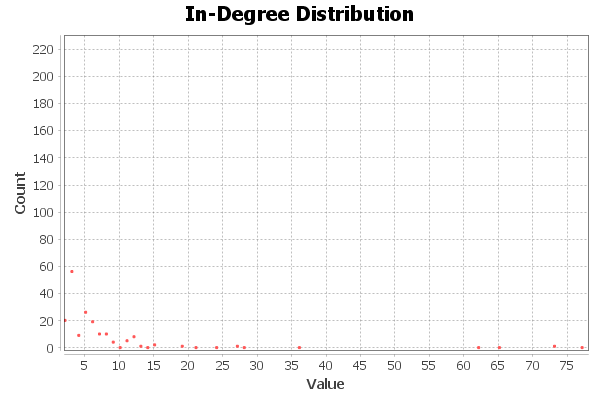
\includegraphics[width=12cm]{../images/in-degree-distribution}
	\caption{Distribución de grados de entrada para la red filtrada}
	\label{fig:in-degree-distribution}
\end{figure}

\begin{figure}[H]
	\centering
	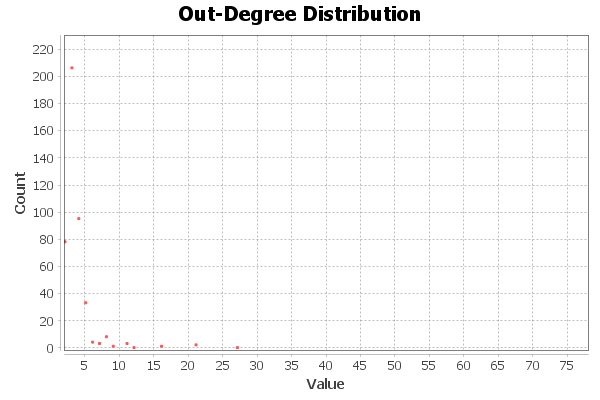
\includegraphics[width=12cm]{../images/out-degree-distribution}
	\caption{Distribución de grados de salida para la red filtrada}
	\label{fig:out-degree-distribution}
\end{figure}

Se puede observar como se cumple la ley de la potencia: $ P(k) \sim k^{-\gamma} $ y es que la mayoría de los nodos tienen pocos enlaces pero hay unos cuantos \textit{hubs} que tienen muchos, y posteriormente, al visualizarlo se verá una forma de estrella alrededor de estos. Por tanto podríamos decir que la red es libre de escala.

\subsection{Distribución de distancias}

\begin{figure}[H]
	\centering
	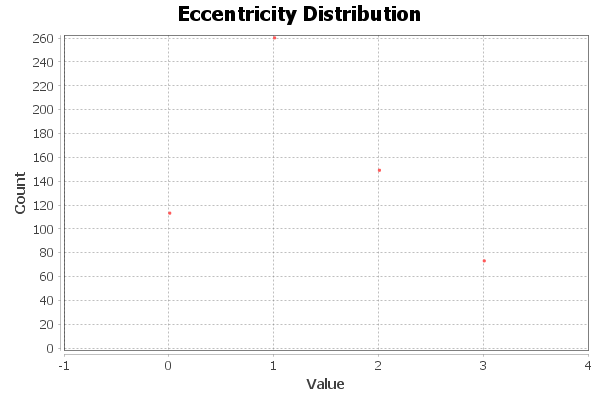
\includegraphics[width=12cm]{../images/eccentricity-distribution}
	\caption{Distribución de excentricidad para la red filtrada}
	\label{fig:eccentricity-distribution}
\end{figure}

En este gráfico (Figura \ref{fig:eccentricity-distribution}) vemos que hay bastantes nodos con distancia 0, esto es porque en el grafo hay nodos con grado de salida 0 y al ser una red dirigida es imposible llegar a ellos.
\\ \\
Recordamos, el diámetro de la red era 3 y la distancia media 1,431. En la distribución vemos como a mayor sea el valor de distancia, menor es el número de nodos. Esto es consecuencia de cumplir la propiedad de mundo pequeño. 

\subsection{Distribución de coeficientes de clustering}

El coeficiente de clustering de la red social es bastante bajo, de hecho en la red filtrada da un valor de 0 y en la red sin filtrar 0,074.
\\ \\

\section{Medidas de centralidad para nodos principales}
\label{sec:hubs}

En esta sección se va a intentar detectar a los actores principales dentro de la red social utilizando el numero de followers.
\\ \\

\begin{table}[H]
	\centering
	\caption{Actores principales según sus followers}
	\label{tab:actores-principales-grado}
	\begin{tabular}{| l | l l |}
		\hline
		\# & \textit{User}       & \textit{Followers}    \\
		\hline
1 & @el\_pais           & 6656276 \\
2 & @elmundoes         & 3147577 \\
3 & @pablo\_iglesias\_   & 2297480 \\
4 & @\_anapastor\_       & 2022272 \\
5 & @a3noticias        & 1701612 \\
6 & @marianorajoy      & 1659831 \\
7 & @abc\_es            & 1551931 \\
8 & @antena3com        & 1366042 \\
9 & @20m               & 1365736 \\
10 & @ahorapodemos      & 1333177 \\
11 & @la\_ser            & 1154019 \\
12 & @sextanoticias     & 1081235 \\
13 & @europapress       & 1059152 \\
14 & @albert\_rivera     & 1034997 \\
15 & @publico\_es        & 899461  \\
16 & @sanchezcastejon   & 788591  \\
17 & @elconfidencial    & 746203  \\
18 & @antoniobanderas   & 691916  \\
19 & @alexdelaiglesia   & 504784  \\
20 & @diostuitero       & 457414  \\ 
		\hline
	\end{tabular}
\end{table}

\section{Comunidades}

Se ha utilizado Gephi para detectar comunidades dando una resolución de 1,5 y obteniendo 11 comunidades y un coeficiente de 0,727, el cual supera la barrera de 0,3 para considerarlo aceptable.
\\ \\

\begin{figure}[H]
	\centering
	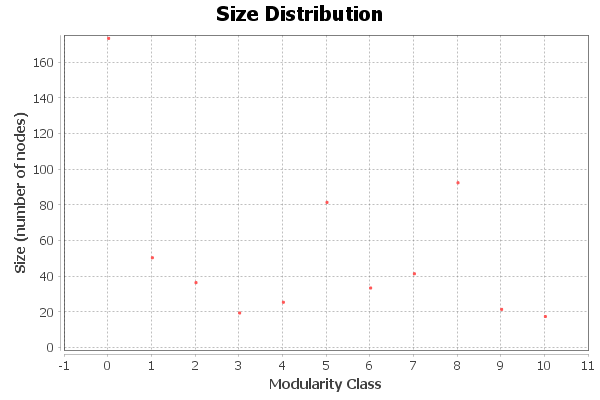
\includegraphics[width=12cm]{../images/communities-size-distribution}
	\caption{Distribución de comunidades en la red filtrada}
	\label{fig:communities-size-distribution}
\end{figure}

\begin{figure}[H]
	\centering
	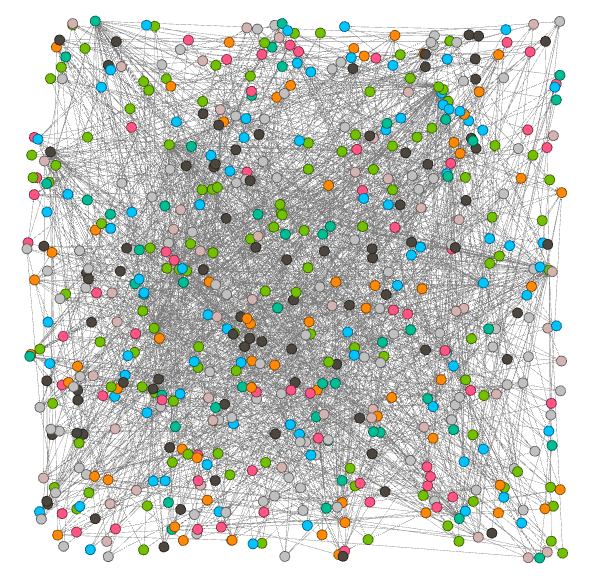
\includegraphics[width=12cm]{../images/modularity-class}
	\caption{Grafo de comunidades en la red filtrada}
	\label{fig:modularity-class}
\end{figure}

\section{Visualización}

\begin{figure}[H]
	\centering
	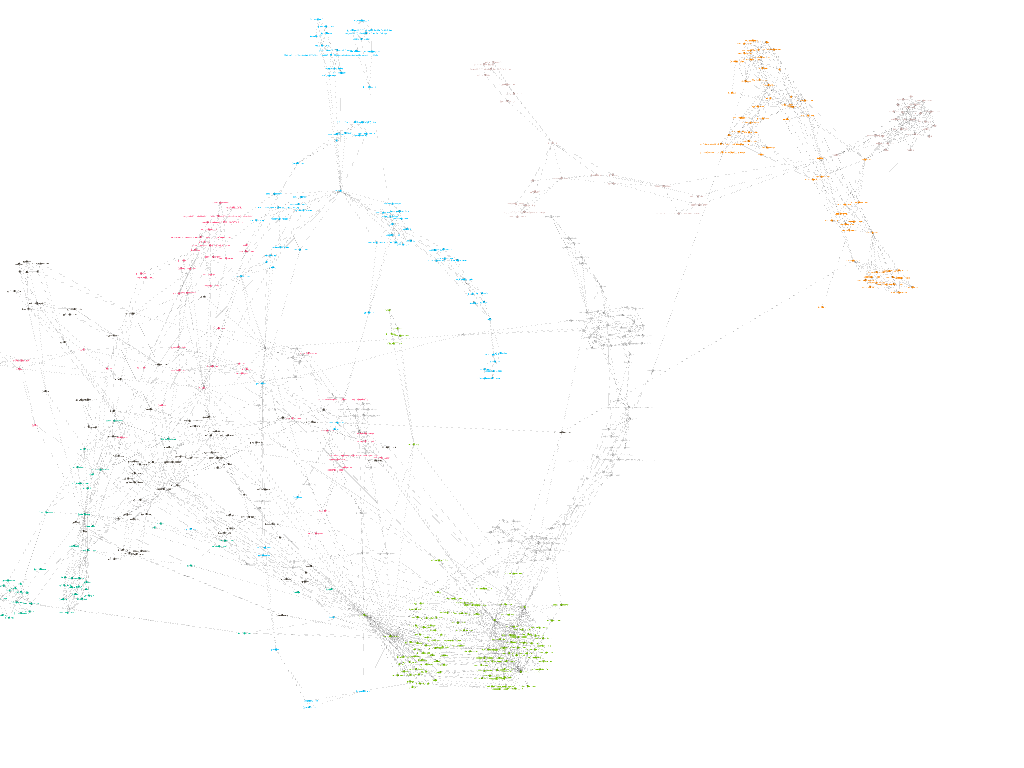
\includegraphics[width=14cm]{../images/atlas}
	\caption{Visualización utilizando Force Atlas}
\end{figure}

Para testear una red con comunidad más pequeña se incrementó el valor del K-Core a 5, dándonos una red de 55 nodos y 211 aristas, en la que se puede apreciar que usuarios fueron los mas comentados, estableciéndose una comunidad de tamaño 2.

\begin{figure}[H]
	\centering
	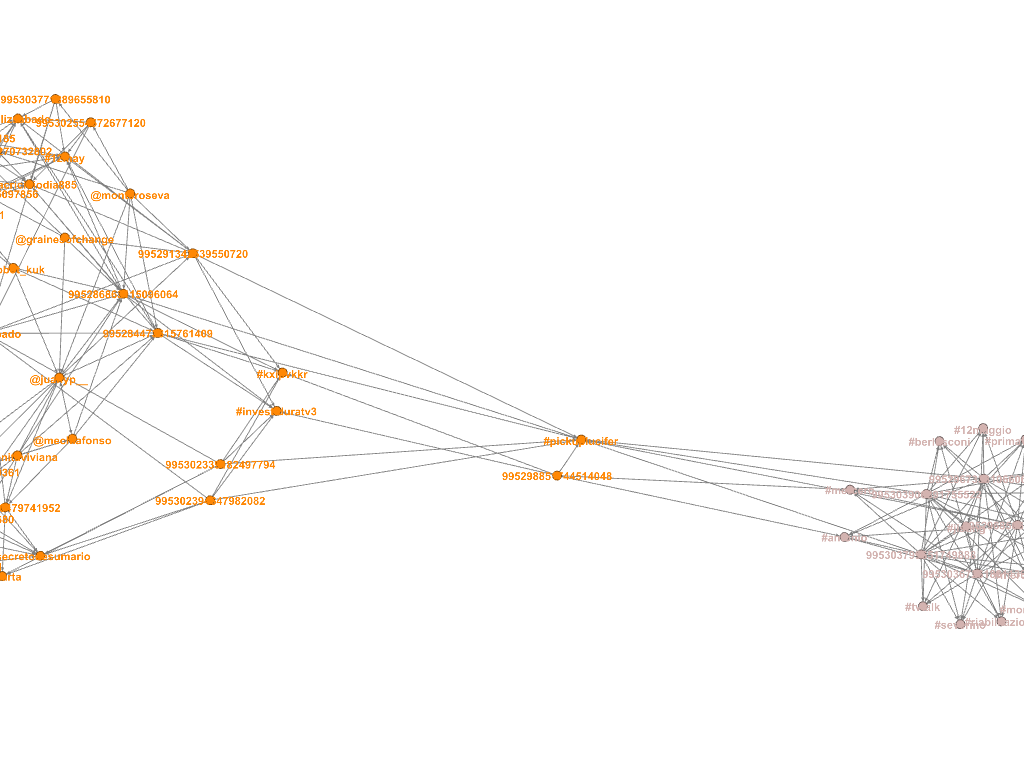
\includegraphics[width=14cm]{../images/atlas2}
	\caption{Visualización utilizando Force Atlas aumentando el K-core a 5}
\end{figure}

\begin{figure}[H]
	\centering
	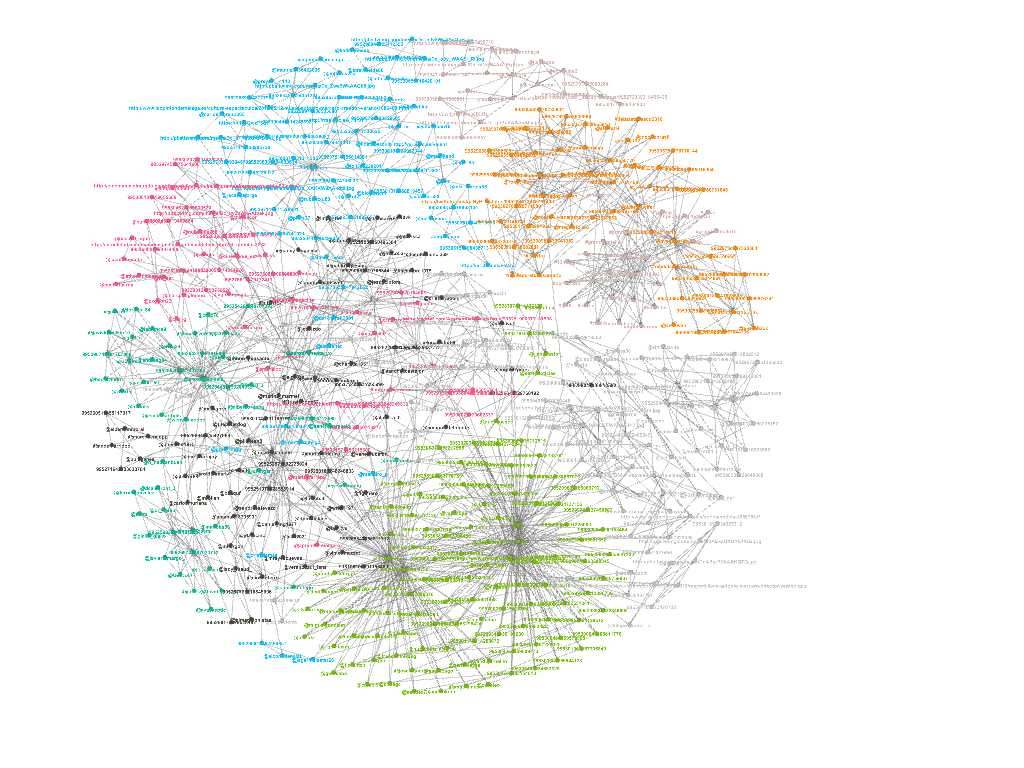
\includegraphics[width=14cm]{../images/fruchterman-reingold}
	\caption{Visualización utilizando el algoritmo de Fruchterman Reingold}
	\label{fig:fruchterman-reingold}
\end{figure}

Se han probado los dos algoritmos principales para visualizar las redes (de distribución guiados por fuerzas), en primer lugar el de Fruchterman Reingold usando el número de seguidores para el tamaño del nodo y la comunidad a la que pertenece para el color (Figura \ref{fig:fruchterman-reingold}).
	
\begin{figure}[H]
	\centering
	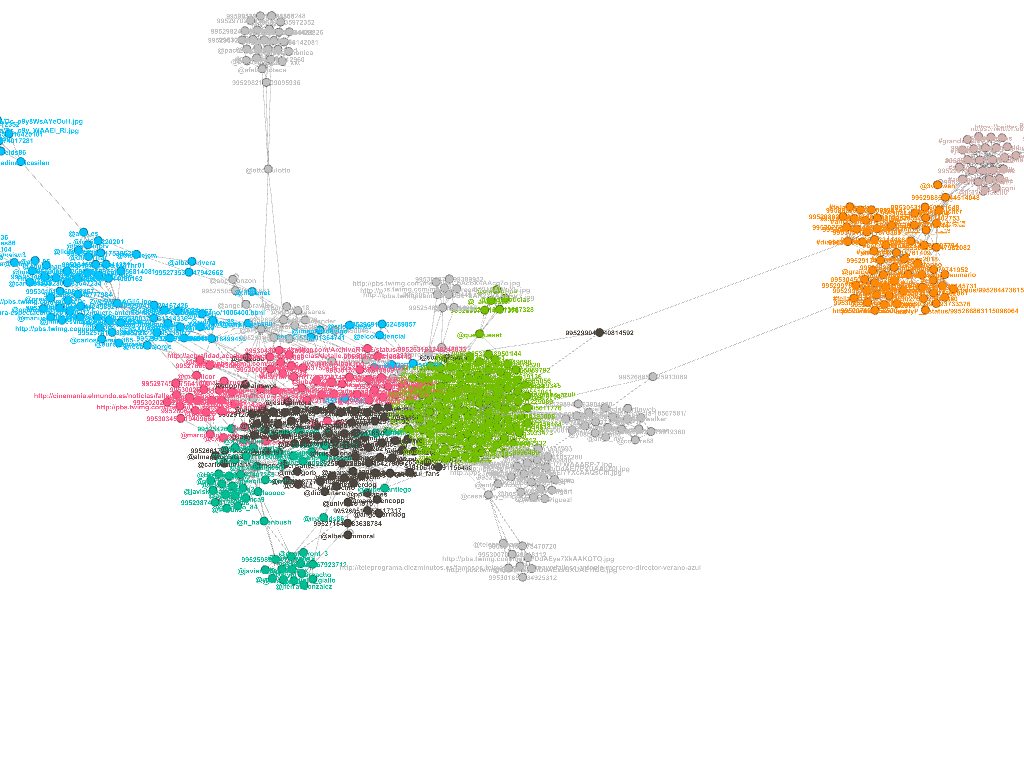
\includegraphics[width=14cm]{../images/kamada-kawai}
	\caption{Visualización utilizando el algoritmo de Kamada Kawai}
	\label{fig:kamada-kawai}
\end{figure}


También se ha probado el de Kamada Kawai (\textit{Force Atlas 2} en Gephi) usando el número de seguidores para el tamaño del nodo y la comunidad a la que pertenece para el color (Figura \ref{fig:kamada-kawai}).

\bigskip
Viendo sendas visualizaciones, me parece que aporta más la segunda. Separa muy bien dos comunidades que se alejan bastante del núcleo y dentro de éste la mayoría de los nodos de una misma comunidad están en el centro, excepto los más centrales donde se mezclan de varias comunidades (tal vez porque podrían pertenecer perfectamente a cualquiera).
